% Drawing 154/09-15 -- folder 154, batch 09, archive page 175 (PDF page 176).
% Transcription: au-dessous, les positions successives de ce cycle : une droite rouge horizontale coupée d'un croisement de deux droites rouges et de deux droites verticales rouges ; une droite vert clair et des droites en tirets vert foncé, gris et bleu qui passent au-dessus ou au-dessous du croisement, leurs extrémités marquées $3$, $5 = 1$, $4$ et $2$, avec une flèche. À côté, deux cercles bleus autour de deux croisements, reliés par un arc. À droite, un disque traversé de pseudo-droites rouges, triangles coloriés en jaune, une bande en tirets rouges. En bas à gauche, un trèfle de trois disques bordés de vert clair, traversés de pseudo-droites rouges, secteurs coloriés en jaune, les bords marqués $D_0$, $D_1$ en alternance ; au crayon, un disque sur lequel un petit segment vert porte deux cercles, et des ovales. Au milieu, un croquis de coins vert clair et vert foncé réunis par des traits. En bas à droite, une droite vert clair coupée de droites rouges, en partie en tirets, et d'une droite oblique rouge, deux segments de la droite verte noircis, des hachures au crayon
% Kind: page of figures: cycle of positions, clover of three disks, line cut by lines. Method 2 (redraw from the facsimile). Status: partial.
% Notes: Redrawn from a 400 dpi colour crop, coordinates read on gridded crops and the redraw checked on an overlay. Seven figures. Top left: the red horizontal line with its arrowhead and the label 2; two red lines crossing on it in one point; two red verticals; two light green lines that step down from left to right, the upper one (end marked 3) passing over the crossing and down between the verticals, the lower one (end marked 5 = 1) passing through the crossing; two dark green dashed lines beside them, one blue dashed line that runs under the red line and passes above it at the first vertical; a black wavy stroke on the red line between the crossing and the first vertical, a pencil rotation arrow under it, the label 4 with its arrow. Top: two pencil circles, each round the crossing of a red vertical with the red horizontal, their facing halves thickened in blue, a blue dashed stroke between them and a pencil rotation arrow. Right: the disk with its light green rim, a dark green stroke at the top and one at the lower left, black dots along the bottom, seven red strands from rim to rim, one red dashed strand, twelve yellow regions. Bottom left: the clover of three light green circles, the two lower ones bounded by dark arcs towards the middle, blue strokes at the two corners and blue dots along the two bottoms, the red strands, eighteen yellow regions, the letters D_0, D_1 round each circle and alpha, beta at the centre (twice more in pencil), four small pencil triangles; under it two pencil ovals. Left: the pencil disk with a dashed equator, a light green segment carrying two small black circles. Middle: a light green bar and two small light green boxes joined by dark green strokes, blue strokes, pencil arcs. Bottom right: the light green line, the oblique red line through it, two red lines crossing on the oblique in one point, four more red lines, four red dashed lines, two blackened pieces of the green line each with a triangle hatched in pencil up to the oblique. Below the middle, a large pencil circle. Still approximate: in the clover the strands are followed where they overlap and their crossings inside each disk are not computed vertex by vertex, so the yellow regions are placed by eye; in the right-hand disk the red dashed strand and the small central regions; the faint pencil hatching on either side of the bottom right figure and the faint pencil curves round the middle sketch are not drawn. Redrawn 2026-11-12 (issue 128): to check again.
% Coordinates: 1 unit = 1 mm = 1/100 of the crop width (bbox in page fractions: [0.13, 0.1, 0.97, 0.535]).
% Redrawn by Claude (claude-fable-5-2), issue #128, 2026-11-12, from a 400 dpi colour crop of the facsimile and checked on an overlay; not checked by a human; not compiled (no TeX in the session).
% Rights: reproduces part of the work -- behind RENDER_TRANSCRIPTS, never published by itself.
\documentclass[tikz,border=3pt]{standalone}
\usepackage{amsmath,amssymb}
\usetikzlibrary{patterns,arrows.meta}
\tikzset{Or/.style={orange!90!black}, Re/.style={red!85!black}, Ye/.style={yellow!80!orange}, Lg/.style={green!60!black!70}, Dg/.style={green!45!black}, Br/.style={brown!70!black}, Bl/.style={blue!70!black}, Gy/.style={black!40}, pencil/.style={black!45}, struck/.style={black!35}, mpt/.style={circle,draw,inner sep=1.3pt}, pt/.style={circle,fill,inner sep=0.9pt}, opt/.style={circle,draw,fill=white,inner sep=1.1pt}}
\begin{document}
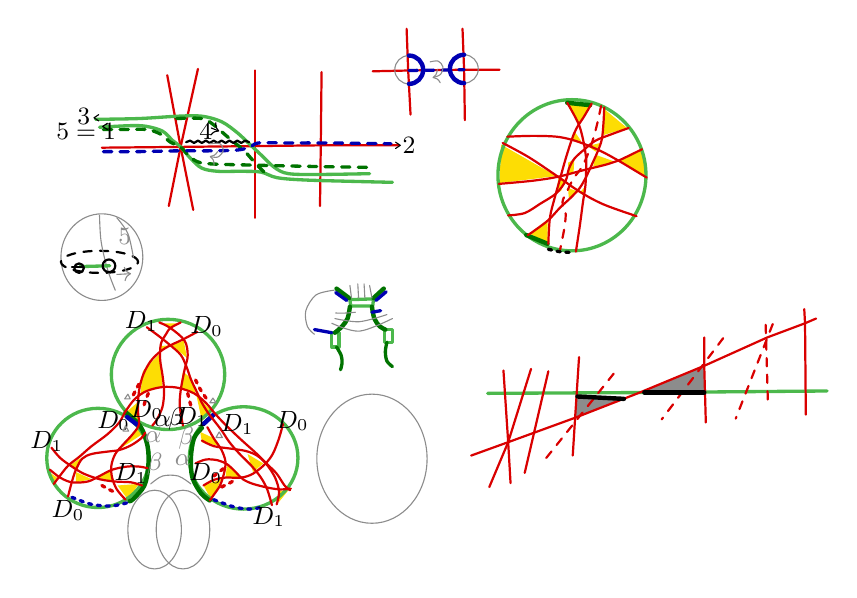
\begin{tikzpicture}[x=1mm,y=1mm,line cap=round,line join=round,font=\small]
\draw[Re,thick] (7.3,-19.1) -- (17.3,-19) -- (26.7,-18.9) -- (35.1,-18.8) -- (45,-18.8);
\draw[black] (44.6,-18.4) -- (45.2,-18.8) -- (44.6,-19.2);
\node[inner sep=1pt] at (46.3,-18.8) {$2$};
\draw[Re,thick] (15.6,-9.9) -- (17.3,-19) -- (18.9,-27);
\draw[Re,thick] (19.5,-9.1) -- (17.3,-19) -- (15.8,-26.5);
\draw[Re,thick] (26.7,-9.3) -- (26.7,-18.9) -- (26.7,-28);
\draw[Re,thick] (35.2,-9.5) -- (35.1,-18.8) -- (35,-26.5);
\draw[Lg,very thick] plot[smooth, tension=0.55] coordinates {(6.5,-15.5) (12,-15.4) (17,-15.1) (20,-15.1) (22.5,-15.8) (24.5,-17.2) (26,-18.6) (27.5,-20) (29.2,-21.6) (31,-22.4) (35,-22.5) (41.3,-22.4)};
\draw[Lg,very thick] plot[smooth, tension=0.55] coordinates {(7,-16.5) (11,-16.3) (13,-16.4) (15,-17) (16.3,-18.2) (17.3,-19) (18.6,-20.5) (20,-21.7) (22,-22.1) (25,-22.1) (27.5,-22.2) (29.5,-22.9) (33,-23.2) (40,-23.4) (44.2,-23.5)};
\draw[Dg,very thick,dashed] plot[smooth, tension=0.55] coordinates {(16.8,-15.4) (20,-15.4) (21.5,-16.2) (23,-17.5) (24.2,-18.5) (25.3,-19.4) (26.2,-20.4) (27,-21.3) (28,-22.3)};
\draw[Dg,very thick,dashed] plot[smooth, tension=0.55] coordinates {(7.5,-16.8) (10,-16.8) (13,-16.8) (14.8,-17.4) (16,-18.4) (17.3,-19) (18.5,-20.3) (19.8,-21) (22,-21.2) (26,-21.3) (30,-21.4) (35,-21.5) (41,-21.6)};
\draw[Bl,very thick,dashed] plot[smooth, tension=0.55] coordinates {(7.5,-19.6) (12,-19.6) (17,-19.5) (21,-19.5) (24.5,-19.4) (26.2,-19) (27.2,-18.5) (31,-18.5) (36,-18.5) (44,-18.6)};
\draw[black,thick] (18,-18.4) -- (18.5,-18.2) -- (19,-18.5) -- (19.5,-18.2) -- (20,-18.5) -- (20.5,-18.2) -- (21,-18.5) -- (21.5,-18.2) -- (22,-18.5) -- (22.5,-18.2) -- (23,-18.5) -- (23.5,-18.2) -- (24,-18.5) -- (24.5,-18.2) -- (25,-18.5) -- (25.5,-18.2) -- (26,-18.4);
\draw[pencil,->] plot[smooth, tension=0.55] coordinates {(21,-18.6) (22.3,-18.6) (22.7,-19.5) (22,-20.3) (21,-20.2)};
\draw[black] (6.9,-14.9) -- (6.3,-15.3) -- (6.9,-15.7);
\node[inner sep=1pt] at (5,-15.2) {$3$};
\draw[black] (8,-16) -- (7.4,-16.4) -- (8,-16.8);
\node[inner sep=1pt] at (5.3,-17) {$5=1$};
\node[inner sep=1pt] at (20.5,-17) {$4$};
\draw[black,->] (21.2,-16.6) -- (22.2,-17);
\draw[Re,thick] (41.7,-9.4) -- (46.2,-9.3) -- (53.3,-9.2) -- (57.8,-9.2);
\draw[Re,thick] (46,-4) -- (46.2,-9.3) -- (46.5,-14.9);
\draw[Re,thick] (53.1,-4) -- (53.3,-9.2) -- (53.4,-15.6);
\draw[pencil] (46.3,-9.2) circle[radius=1.8];
\draw[pencil] (53.3,-9.1) circle[radius=1.8];
\draw[Bl,ultra thick] (46.3,-7.4) arc[start angle=90, end angle=-90, radius=1.8];
\draw[Bl,ultra thick] (53.3,-7.3) arc[start angle=90, end angle=270, radius=1.8];
\draw[Bl,very thick,dashed] (46.3,-9.3) -- (53.3,-9.2);
\draw[pencil,->] plot[smooth, tension=0.55] coordinates {(49,-8.2) (50,-8.1) (50.6,-8.8) (50.3,-9.8) (49.3,-10.2)};
\fill[pattern=north east lines,Ye] (66.6,-13.6) -- (69.3,-13.8) -- (67.9,-16) -- cycle;
\fill[pattern=north east lines,Ye] (71.1,-14.2) -- (74,-16.6) -- (71,-17.5) -- cycle;
\fill[pattern=north east lines,Ye] (73,-20.8) -- (76,-19.4) -- (76.4,-22.8) -- cycle;
\fill[pattern=north east lines,Ye] (58,-18.7) -- (65,-22.7) -- (57.8,-23.6) -- cycle;
\fill[pattern=north east lines,Ye] (61.6,-30) -- (63.9,-28.3) -- (63.9,-31.2) -- cycle;
\fill[pattern=north east lines,Ye] (67.3,-17) -- (68.2,-18.3) -- (67,-18.2) -- cycle;
\fill[pattern=north east lines,Ye] (69,-18.9) -- (70.6,-18.5) -- (70,-19.6) -- cycle;
\fill[pattern=north east lines,Ye] (70,-20) -- (72.5,-20.9) -- (69.7,-21.5) -- cycle;
\fill[pattern=north east lines,Ye] (66.5,-21) -- (67.3,-20.6) -- (67.2,-22.3) -- (66.6,-22.5) -- cycle;
\fill[pattern=north east lines,Ye] (65.3,-22.9) -- (66.2,-23.2) -- (65.6,-24.6) -- (65,-24.8) -- cycle;
\fill[pattern=north east lines,Ye] (66.5,-24.2) -- (67.8,-24.7) -- (66.6,-25.5) -- cycle;
\fill[pattern=north east lines,Ye] (68,-24.8) -- (68.7,-24) -- (68.5,-25.2) -- cycle;
\draw[Lg,very thick] (67,-22.6) ellipse[x radius=9.4, y radius=9.6];
\draw[Dg,ultra thick] (66.4,-13.4) -- (69.3,-13.7);
\draw[Dg,ultra thick] (61.2,-30.2) -- (63.9,-31.3);
\draw[black,very thick,dotted] plot[smooth, tension=0.55] coordinates {(64,-32) (65.4,-32.3) (66.8,-32.4)};
\draw[Re,thick] plot[smooth, tension=0.55] coordinates {(58.8,-17.7) (62,-17.6) (65,-17.7) (67,-18.1) (69,-18.8) (71,-19.7) (73,-20.8) (75,-22) (76.5,-22.9)};
\draw[Re,thick] plot[smooth, tension=0.55] coordinates {(58.2,-18.5) (61.5,-20.3) (65.1,-22.7) (68,-24.7) (71,-26.3) (75.2,-27.8)};
\draw[Re,thick] plot[smooth, tension=0.55] coordinates {(57.7,-23.7) (62,-23.3) (65.2,-22.8) (68.3,-22) (71.5,-21.2) (73,-20.7) (75.9,-19.3)};
\draw[Re,thick] plot[smooth, tension=0.55] coordinates {(58.9,-27.7) (61,-27.4) (63,-26.2) (65,-24.9) (66.2,-23.3) (66.6,-21.8) (67.3,-20.5) (68.6,-19.3) (70,-18.2) (72,-17.4) (74.2,-16.6)};
\draw[Re,thick] plot[smooth, tension=0.55] coordinates {(66.4,-13.4) (67.3,-15) (68,-16.5) (68.5,-18.5) (68.8,-20.5) (68.8,-22) (68.7,-24) (68.4,-26) (68,-29) (67.5,-32.3)};
\draw[Re,thick] plot[smooth, tension=0.55] coordinates {(69.5,-13.5) (68.5,-15.2) (67.6,-16.6) (67,-18) (66.2,-20.5) (65.5,-23) (64.8,-25.5) (64.2,-28) (64,-31.3)};
\draw[Re,thick] plot[smooth, tension=0.55] coordinates {(71.1,-14) (71,-16) (70.8,-18) (70.3,-19.5) (69.5,-21.3) (68.8,-22.8) (68,-24.2) (66.8,-25.5) (65.5,-26.7) (64,-28.3) (62,-29.8) (61.4,-30.2)};
\draw[Re,thick,dashed] plot[smooth, tension=0.55] coordinates {(70.7,-13.8) (70.1,-16.5) (69.3,-19.2) (68.3,-21.5) (67.2,-23) (66.4,-24.6) (65.8,-26) (66.2,-27.5) (66,-29.5) (65.5,-32)};
\fill[pattern=north east lines,Ye] (12.5,-47.5) -- (14.7,-45.2) -- (15,-49.5) -- (12.2,-50.3) -- cycle;
\fill[pattern=north east lines,Ye] (17.6,-47.5) -- (18.7,-48.5) -- (19.2,-50.3) -- (17.3,-49.6) -- cycle;
\fill[pattern=north east lines,Ye] (16.2,-44.2) -- (17.7,-43.6) -- (18.1,-45.8) -- cycle;
\fill[pattern=north east lines,Ye] (14.7,-44.3) -- (15.9,-44.2) -- (14.8,-45) -- cycle;
\fill[pattern=north east lines,Ye] (15.1,-41.4) -- (16.8,-41.4) -- (16,-42) -- cycle;
\fill[pattern=north east lines,Ye] (10.5,-52.6) -- (12,-51.3) -- (12,-53.8) -- cycle;
\fill[pattern=north east lines,Ye] (19.3,-50.5) -- (21.3,-52.6) -- (20,-53.8) -- cycle;
\fill[pattern=north east lines,Ye] (9.2,-57.6) -- (12.4,-55.5) -- (12,-54.6) -- (10.5,-56.3) -- cycle;
\fill[pattern=north east lines,Ye] (3.3,-59.4) -- (4.6,-58.5) -- (4.2,-60) -- cycle;
\fill[pattern=north east lines,Ye] (4,-60.3) -- (6,-61.2) -- (4,-61.6) -- cycle;
\fill[pattern=north east lines,Ye] (6.5,-61) -- (8.5,-60) -- (8.6,-61.4) -- cycle;
\fill[pattern=north east lines,Ye] (9.3,-62) -- (12,-61.8) -- (10.6,-63.8) -- cycle;
\fill[pattern=north east lines,Ye] (0.6,-60.3) -- (1.6,-61) -- (1,-61.8) -- cycle;
\fill[pattern=north east lines,Ye] (19.8,-55.2) -- (21.5,-56) -- (22.3,-57) -- (20,-56.5) -- cycle;
\fill[pattern=north east lines,Ye] (25.8,-58) -- (27.8,-59.2) -- (26.5,-60.3) -- cycle;
\fill[pattern=north east lines,Ye] (23.2,-59.3) -- (25,-61) -- (23,-61) -- cycle;
\fill[pattern=north east lines,Ye] (20.2,-62) -- (22.5,-61.2) -- (21.2,-63.8) -- cycle;
\fill[pattern=north east lines,Ye] (29.8,-62.7) -- (31,-62.6) -- (29.7,-64.2) -- cycle;
\draw[Lg,very thick] (15.7,-47.9) ellipse[x radius=7.2, y radius=7];
\draw[Lg,very thick] (6.8,-58.5) ellipse[x radius=6.5, y radius=6.3];
\draw[Lg,very thick] (25.3,-58.5) ellipse[x radius=6.9, y radius=6.5];
\draw[Dg,ultra thick] plot[smooth, tension=0.55] coordinates {(10.3,-52.7) (12.2,-54.5) (13.1,-57) (13.2,-59.5) (12.7,-62) (11.3,-63.7) (10.8,-64)};
\draw[Dg,ultra thick] plot[smooth, tension=0.55] coordinates {(20,-54.7) (19,-56) (18.6,-58.5) (18.8,-61) (19.9,-63) (21,-63.9)};
\draw[Bl,ultra thick] (10.5,-53.3) -- (11.8,-54.3);
\draw[Bl,ultra thick] (20.2,-54.2) -- (21.5,-53);
\draw[Bl,very thick,dotted] plot[smooth, tension=0.55] coordinates {(3.5,-63.5) (6,-64.4) (8.5,-64.6) (10.5,-64.2)};
\draw[Bl,very thick,dotted] plot[smooth, tension=0.55] coordinates {(21.5,-63.8) (24,-64.7) (26,-65) (28,-64.7)};
\draw[Re,thick] plot[smooth, tension=0.55] coordinates {(14.6,-41.3) (16,-42) (17.8,-43.6) (18.2,-45.5) (17.8,-47.3) (17.3,-50) (17.2,-52) (17.6,-54.4)};
\draw[Re,thick] plot[smooth, tension=0.55] coordinates {(17.3,-41.3) (16,-42) (15.5,-42.7) (14.8,-44) (14.7,-46) (15,-48) (15.2,-50) (15,-52) (14.3,-53.6) (13.7,-54.4)};
\draw[Re,thick] plot[smooth, tension=0.55] coordinates {(13,-41.9) (14.5,-43) (16,-44.2) (17.3,-45.4) (18,-46.8) (18.6,-48.5) (19.3,-50) (20,-51.5) (20.8,-52.8) (21.5,-53.7) (22.5,-55) (23.5,-56.5) (24.8,-58) (26.3,-59.5) (27.5,-61) (28.3,-62.5) (28.9,-64.5)};
\draw[Re,thick] plot[smooth, tension=0.55] coordinates {(19.4,-42.5) (17.5,-43.5) (16,-44.2) (14.7,-45) (13.5,-46.2) (12.6,-47.8) (12.1,-49.5) (11.9,-51.2) (11.9,-52.8) (12,-54.3) (11.2,-55.5) (10,-56.8) (9,-58) (8.5,-59.5) (8.6,-61) (9.2,-62.5) (10.3,-63.8)};
\draw[Re,thick] plot[smooth, tension=0.55] coordinates {(1.2,-61.8) (1.8,-61) (3,-59.5) (4.5,-58.3) (6,-57) (8,-55.5) (9.5,-54) (10.3,-52.6) (11.5,-51) (13,-50) (15,-49.5) (17,-49.6) (19,-50.3) (20.5,-51.5) (21.6,-52.8) (23,-54.3) (25,-56.2) (27,-58) (28.3,-59.3) (29.5,-60.5) (30.5,-62) (31.2,-62.6)};
\draw[Re,thick] plot[smooth, tension=0.55] coordinates {(0.9,-57.2) (2,-58.5) (3.5,-59.6) (5,-60.5) (7,-61.2) (9,-61.5) (11,-61.6) (12.4,-62)};
\draw[Re,thick] plot[smooth, tension=0.55] coordinates {(0.7,-60) (2,-61) (3.5,-61.6) (5.5,-61.5) (7,-60.8) (8.6,-60) (10.5,-59.6) (12,-59.6) (13.1,-59.8)};
\draw[Re,thick] plot[smooth, tension=0.55] coordinates {(3,-63.4) (3.5,-61.5) (4,-60) (4.8,-58.6) (6,-58) (8,-57.7) (9.5,-57.5) (11,-56.9) (12.3,-56) (12.8,-55.3)};
\draw[Re,thick] plot[smooth, tension=0.55] coordinates {(30.3,-54.2) (29.8,-56) (29,-58) (28,-59.3) (26.5,-60.5) (25,-61) (23,-61) (21.5,-61.3) (20.2,-62)};
\draw[Re,thick] plot[smooth, tension=0.55] coordinates {(19.2,-59.2) (20.5,-58.7) (22,-58.8) (23.2,-59.3) (24.3,-60.3) (25.2,-61.2) (26.5,-61.8) (28.5,-62.3) (30,-62.5) (31.3,-62.4)};
\draw[Re,thick] plot[smooth, tension=0.55] coordinates {(20,-56.3) (21.5,-57) (23.5,-57.3) (25.5,-57.6) (27,-58.2) (28.2,-59.3) (29.3,-61) (29.8,-62.8) (29.5,-64.4)};
\draw[Re,thick] plot[smooth, tension=0.55] coordinates {(20.7,-54.6) (21.5,-56) (22.5,-57.5) (23,-59) (22.8,-60.5) (22.3,-62) (21.5,-63.2) (21,-63.9)};
\draw[Re,very thick,dotted] plot[smooth, tension=0.55] coordinates {(11.3,-50.5) (11.8,-49.5) (12.1,-49)};
\draw[Re,very thick,dotted] plot[smooth, tension=0.55] coordinates {(13.2,-50.3) (12.8,-51.3) (12.6,-52)};
\draw[Re,very thick,dotted] plot[smooth, tension=0.55] coordinates {(18.2,-50.3) (18.5,-51.5) (18.7,-52.2)};
\draw[Re,very thick,dotted] plot[smooth, tension=0.55] coordinates {(19.2,-48.6) (19.8,-49.8) (20.6,-51)};
\draw[Re,very thick,dotted] plot[smooth, tension=0.55] coordinates {(7.3,-62) (8.2,-62.5) (9,-62.9)};
\draw[Re,very thick,dotted] plot[smooth, tension=0.55] coordinates {(21.5,-60.8) (22.3,-60.2) (22.8,-59.8)};
\draw[Re,very thick,dotted] plot[smooth, tension=0.55] coordinates {(22.5,-62.2) (23.5,-61.7) (24.2,-61.3)};
\node[inner sep=1pt] at (12.3,-41.2) {$D_1$};
\node[inner sep=1pt] at (20.6,-41.8) {$D_0$};
\node[inner sep=1pt] at (13,-52.4) {$D_0$};
\node[inner sep=1pt] at (18.7,-53.3) {$D_1$};
\node[inner sep=1pt] at (8.8,-53.8) {$D_0$};
\node[inner sep=1pt] at (0.3,-56.4) {$D_1$};
\node[inner sep=1pt] at (3,-65.2) {$D_0$};
\node[inner sep=1pt] at (11,-60.5) {$D_1$};
\node[inner sep=1pt] at (24.5,-54.3) {$D_1$};
\node[inner sep=1pt] at (31.5,-53.8) {$D_0$};
\node[inner sep=1pt] at (20.5,-60.5) {$D_0$};
\node[inner sep=1pt] at (28.5,-66) {$D_1$};
\node[inner sep=1pt] at (15,-53.8) {$\alpha$};
\node[inner sep=1pt] at (16.7,-53.6) {$\beta$};
\node[pencil,inner sep=1pt] at (13.8,-55.8) {$\alpha$};
\node[pencil,inner sep=1pt] at (18,-56) {$\beta$};
\node[pencil,inner sep=1pt] at (14,-59.3) {$\beta$};
\node[pencil,inner sep=1pt] at (17.6,-58.8) {$\alpha$};
\draw[pencil] (10.2,-51) -- (10.9,-51) -- (10.6,-50.4) -- cycle;
\draw[pencil] (21,-51.5) -- (21.8,-51.5) -- (21.4,-50.9) -- cycle;
\draw[pencil] (10,-55.1) -- (10.7,-55.1) -- (10.3,-54.4) -- cycle;
\draw[pencil] (21.8,-55.9) -- (22.6,-55.9) -- (22.2,-55.2) -- cycle;
\draw[pencil] (14,-67.6) ellipse[x radius=3.4, y radius=5];
\draw[pencil] (17.6,-67.6) ellipse[x radius=3.4, y radius=5];
\draw[pencil] plot[smooth, tension=0.55] coordinates {(13.5,-61.8) (15,-60.8) (17,-60.8) (18.6,-61.8)};
\draw[pencil] (7.3,-33) ellipse[x radius=5.2, y radius=5.5];
\draw[black,thick,dashed] (7,-33.6) ellipse[x radius=4.9, y radius=1.4];
\draw[pencil] plot[smooth, tension=0.55] coordinates {(7,-27.7) (7.2,-31) (8,-34.5) (9,-37.2)};
\draw[pencil] plot[smooth, tension=0.55] coordinates {(9.2,-28) (10.6,-30) (11.3,-33)};
\draw[Lg,very thick] (4.5,-34.2) -- (8.3,-34.1);
\draw[black,thick] (4.4,-34.4) circle[radius=0.6];
\draw[black,thick] (8.2,-34.1) circle[radius=0.8];
\draw[black,thick] (3.5,-34.3) -- (5,-34.3);
\node[pencil,inner sep=1pt] at (10.2,-30.4) {$5$};
\draw[pencil,->] (9.2,-35.2) -- (11,-35.1);
\draw[Lg,very thick] (38.8,-38.4) -- (41.8,-38.3) -- (41.7,-39.2) -- (38.9,-39.2) -- cycle;
\draw[Lg,very thick] (36.5,-42.6) -- (37.4,-42.6) -- (37.4,-44.4) -- (36.5,-44.4) -- cycle;
\draw[Lg,very thick] (43.2,-42.2) -- (44.2,-42.2) -- (44.2,-43.8) -- (43.2,-43.8) -- cycle;
\draw[Dg,ultra thick] (37.1,-37) -- (38.7,-38.2);
\draw[Bl,very thick] (37,-37.5) -- (38.4,-38.5);
\draw[Dg,ultra thick] (43.1,-37) -- (41.8,-38.2);
\draw[Bl,very thick] (43.4,-37.4) -- (42.1,-38.5);
\draw[Dg,ultra thick] plot[smooth, tension=0.55] coordinates {(38.8,-39.3) (38.5,-40.8) (37.8,-41.8) (36.9,-42.6)};
\draw[Dg,very thick] plot[smooth, tension=0.55] coordinates {(37.1,-44.4) (37.7,-45.5) (37.8,-46.5) (37.6,-47.3)};
\draw[Dg,ultra thick] plot[smooth, tension=0.55] coordinates {(41.6,-39.3) (41.9,-40.8) (42.6,-41.8) (43.3,-42.2)};
\draw[Dg,very thick] plot[smooth, tension=0.55] coordinates {(43.5,-43.8) (43.3,-45) (43.5,-46.2) (44.2,-46.9)};
\draw[Bl,very thick] (34.3,-42.2) -- (36.5,-42.6);
\draw[Bl,very thick] (41.6,-40) -- (42.7,-39.8);
\draw[pencil] (38.8,-36.6) -- (39,-38.2);
\draw[pencil] (39.8,-36.4) -- (39.9,-38.2);
\draw[pencil] (40.6,-36.4) -- (40.7,-38.2);
\draw[pencil] (41.3,-36.6) -- (41.6,-38.2);
\draw[pencil] plot[smooth, tension=0.55] coordinates {(37,-40.1) (38.3,-40.1) (39.5,-40)};
\draw[pencil] plot[smooth, tension=0.55] coordinates {(36.9,-40.8) (40,-41.2) (43.5,-40.3)};
\draw[pencil] plot[smooth, tension=0.55] coordinates {(36.5,-41.4) (40,-42.4) (44.2,-40.8)};
\draw[pencil] plot[smooth, tension=0.55] coordinates {(36.8,-37.2) (34.5,-37.8) (33.2,-39.8) (33.4,-41.8) (34.3,-42.8)};
\fill[pattern=north east lines,pencil] (67.6,-51) -- (73.5,-51) -- (67.5,-53.3) -- cycle;
\fill[pattern=north east lines,pencil] (76,-50.1) -- (83.8,-50.1) -- (83.8,-46.9) -- cycle;
\draw[Lg,very thick] (56.3,-50.3) -- (75.6,-50.2) -- (99.4,-50);
\draw[Re,thick] (54.2,-58.2) -- (58.9,-56.5) -- (67.4,-53.4) -- (75.6,-50.2) -- (83.8,-46.8) -- (91.8,-43.2) -- (96.6,-41.4) -- (98,-40.8);
\draw[Re,thick] (58.3,-47.4) -- (58.9,-56.5) -- (59.2,-61.7);
\draw[Re,thick] (61.8,-47.2) -- (58.9,-56.5) -- (56.5,-62.2);
\draw[Re,thick] (64,-47.5) -- (61,-60.4);
\draw[Re,thick] (67.9,-45.7) -- (67.4,-53.4) -- (67.1,-58.2);
\draw[Re,thick] (83.8,-43.2) -- (83.8,-46.8) -- (84,-54);
\draw[Re,thick] (96.5,-39.6) -- (96.6,-41.4) -- (96.7,-53);
\draw[Re,thick,dashed] (72.3,-47.8) -- (63.5,-58.8);
\draw[Re,thick,dashed] (86.2,-43.3) -- (78.4,-53.6);
\draw[Re,thick,dashed] (92.5,-41.5) -- (87.8,-53.5);
\draw[Re,thick,dashed] (91.6,-41.6) -- (91.9,-52);
\draw[black,ultra thick] (67.7,-50.7) -- (73.6,-51);
\draw[black,ultra thick] (76.2,-50.2) -- (83.8,-50.2);
\draw[pencil] (41.6,-58.6) ellipse[x radius=7, y radius=8.2];
\end{tikzpicture}
\end{document}
